\chapter{绪论}

\iffalse           %这是注释
\begin{figure}[htp]
	\centering
	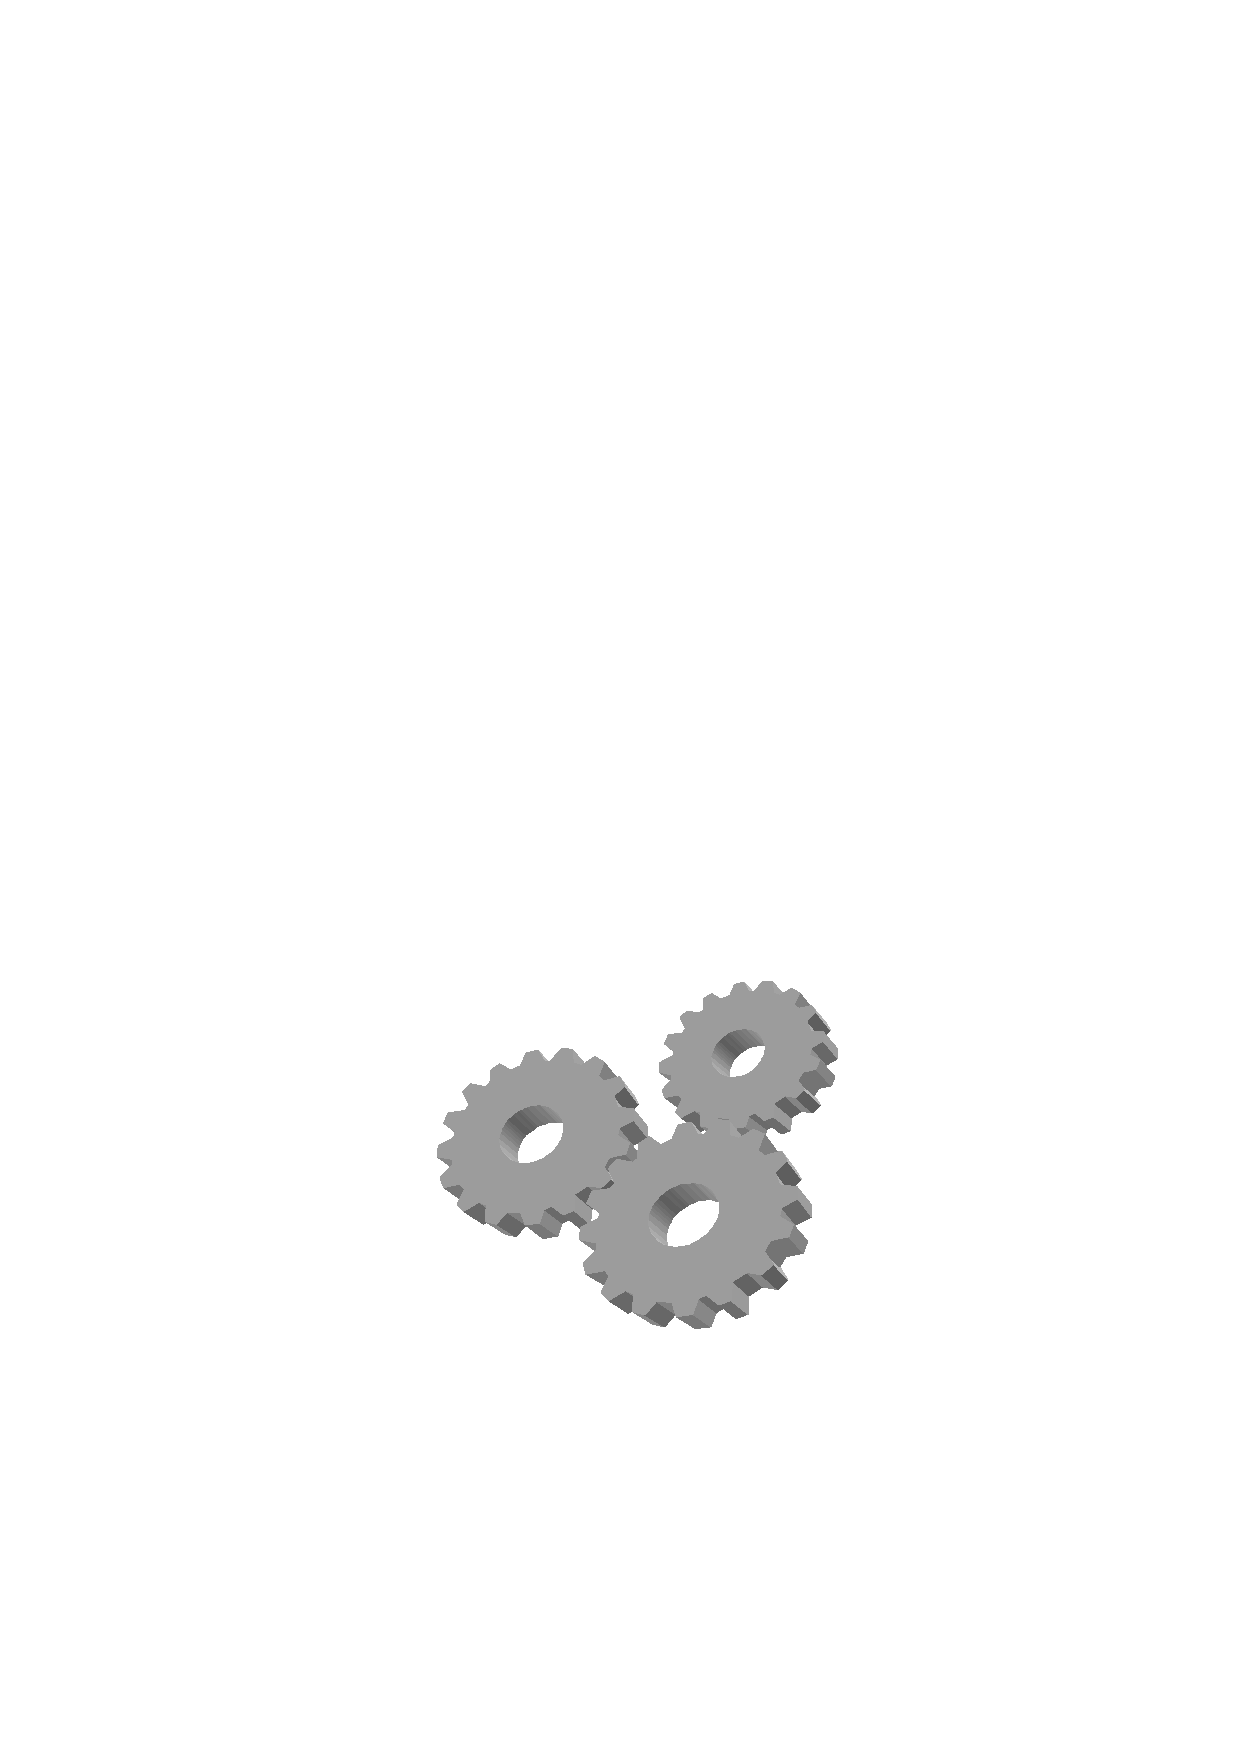
\includegraphics{picmain}
	\caption{图 1.1 名称}
\end{figure}

\begin{table}[htp]
	\centering
	\begin{minipage}[t]{0.8\linewidth} % 如果想在表格中使用脚注,minipage是个不错的办法
		\caption[表 1.1 名称]{}
		\begin{tabular*}{\textwidth}{lp{10cm}}
			\toprule[1.5pt]
			{\hei 列1} & {\hei 列2} \\
			\midrule[1pt]
			&  \\
			& \\
			& \\
			& \\
			& \\
			& \\
			\bottomrule[1.5pt]
		\end{tabular*}
	\end{minipage}
\end{table}


\cite{}

\fi



\section{研究背景与意义}


\subsection{研究背景}
地铁作为现代城市重要的公共交通工具,能够在短时间内运送大量乘客,显著减少城市交通拥堵并提高城市运行效率。然而,随着我国城市化进程的加快,受到公司运营成本、人员流动量大和人员流动速度较快等因素的限制,地铁安检系统面临着日益复杂的挑战,尤其是在防止爆炸物进入地铁环境方面,安检工作仍存在宽松等漏洞。一旦爆炸事件发生,狭窄且封闭的地铁环境极易导致严重的人员伤亡和设备损坏。地下交错复杂的市政设施(如水网、电网)也可能受到严重破坏,从而影响城市正常运行,造成巨大的经济损失和社会混乱。因此,提升地铁环境下的排爆能力对于公共安全和社会稳定至关重要。

传统的地铁排爆工作主要依赖排爆专家等技术人员深入爆炸环境排除爆炸物。然而,传统排爆方法却有很多弊端。
传统的地铁排爆工作主要依赖排爆专家直接进入爆炸现场,手动排除爆炸物。然而,这种方法具有极大的风险性和局限性。首先,排爆专家的生命安全无法得到有效保障,一旦发生爆炸事故,可能导致严重伤亡。其次,地铁内部环境复杂且空间狭窄,传统的手动排爆操作受限于地形条件,尤其是在排椅、扶杆等结构物体较为集中的区域,行动受阻严重。此外,人工操作的排爆效率较低,无法迅速应对紧急情况。

随着机器人技术的迅猛发展,智能救援机器人在地铁排爆任务中的应用逐渐成为研究热点。相较于传统的人工排爆方式,救援机器人在排爆上展现出了诸多优势。救援机器人具有一定的自主能力,可以代替人类进入危险区域进行排爆作业,极大地降低了人员伤亡的风险。其次,救援机器人体型较小便于在地铁排爆环境中移动,视角较低便于发现座椅下等隐匿的爆炸物,方便快速推进排爆工作。再次,救援机器人可以携带多种传感器和设备,显著提高了对环境的感知能力,从而提升了排爆的效率和准确性,成为排爆工作的重要技术支撑。

为了推动救援机器人在地铁排爆环境中的自主作业,至关重要的一点是提高其对周边环境的感知能力。救援机器人依赖于多种传感器的协同工作来感知和理解环境,包括激光雷达、RGB相机和RGB-D相机等。其中,激光雷达(LiDAR)通过发射激光脉冲并捕捉反射回来的信号,生成精确的三维点云数据。这种传感器技术以其高精度和远距离探测能力广泛应用于机器人导航和环境感知。然而,激光雷达在狭窄的地铁环境中存在几个明显的局限性。首先,激光雷达在近距离内存在盲区,通常无法检测到距离较近的物体,尤其是在复杂且密闭的地铁车厢中,这一局限性对机器人操作的安全性和精度构成了挑战。其次,激光雷达生成的点云数据通常较为稀疏,缺乏颜色和纹理等视觉信息,这对环境的详细语义理解造成了限制。此外,激光雷达的制造和使用成本较高,限制了其在部分低成本应用中的推广。相比之下,RGB相机能够捕获场景中物体丰富的颜色、形状和纹理信息,具有视觉效果直观、数据获取丰富的优点。然而,RGB相机的缺陷在于其无法提供物体的深度信息,无法有效理解场景中的三维结构。这对于像地铁排爆这样的复杂环境来说,是一个重大限制,因为仅依靠颜色和纹理信息,机器人难以准确判断物体的空间位置和距离,尤其是在遮挡、光线变化等复杂条件下。

RGB-D相机则通过集成RGB相机和深度相机的功能,克服了上述单一传感器的局限性。RGB相机负责捕捉彩色图像,深度相机则通过测量每个像素点与相机的距离来生成深度图像。这种多模态传感器能够同时获取彩色信息和空间几何信息,使得救援机器人在狭窄、光照不均的地铁环境中,依然能够获得清晰且精确的环境感知能力。尤其是在地铁排爆任务中,RGB-D相机结合了RGB数据中的纹理信息和深度数据中的空间结构信息,为机器人提供了更丰富的视觉信息,使其能够精确识别并定位隐藏在复杂环境中的爆炸物体,显著提升了任务执行的效率和安全性。

语义分割技术是救援机器人在地铁排爆场景中实现精准环境感知的核心手段之一。与基于边框的目标检测方法相比,语义分割能够提供更加细致的场景解析。目标检测通常依赖于矩形框将目标从场景中分割出来,这种方法虽然能提供目标的大致位置,但其边界不够精确,无法应对复杂、遮挡严重的场景。语义分割则通过为图像中的每个像素分配特定的类别,实现像素级别的精确分类与识别。通过这种细致的图像理解,语义分割技术可以全面理解地铁环境中的结构和布局,从而准确识别和分类图像中的物体,提供丰富的语义信息。在地铁排爆任务中,救援机器人依赖语义分割技术,能够在极其复杂的环境下区分地铁座椅、扶手、墙壁以及潜在的爆炸物。这不仅为机器人自主定位、建图、路径规划和任务决策提供了精确的语义信息,还为提升其应对复杂任务的能力提供了技术保障。

RGB-D语义分割的独特之处在于其数据来源的多模态性。RGB-D数据由彩色图像(RGB)和深度图像(Depth)组成,这两类数据虽然在结构上相似,但在数据内容上存在显著差异:RGB图像主要提供物体的颜色、纹理等视觉信息,而深度图像则捕获场景的三维几何信息 。这种模态差异使得RGB-D数据属于异质数据,它们各自具备不同的优势:RGB信息能够帮助机器人识别物体的视觉特征,而深度信息则能够提供物体之间的空间位置关系。因此,如何有效地融合这两类异质数据,使其互为补充,从而提升语义分割的精度与鲁棒性,成为RGB-D语义分割技术的核心挑战。

现有的研究表明,RGB-D语义分割通过结合视觉与几何信息,可以大大增强机器人对复杂环境的感知能力。对于救援机器人而言,地铁环境中的光线变化、遮挡问题、以及目标物体外观特征的多样性,都会对单一模态的感知能力产生负面影响。而RGB-D语义分割技术通过融合RGB和深度数据,能够在这样的复杂条件下,依然实现高精度的语义理解。本文的研究重点在于如何从RGB-D数据中提取并融合不同模态的特征,利用深度学习的方法,提升救援机器人在地铁排爆场景中的语义分割能力,最终实现对异质数据的高效处理与应用。



\subsection{研究意义}
本文的研究在以下四个方面具有重要意义:

(1)  
构建地铁排爆场景的语义分割数据集:本文首先构建了一个专用于地铁排爆任务的语义分割数据集。该数据集涵盖了从地铁闸机、楼梯到地铁车厢内部的多种常见场景,场景中包含了座椅、扶手、地板等常见物体,并模拟了管状爆炸物的放置。通过对这些典型地铁场景的建模和语义标注,本文的工作为救援机器人的环境感知与任务执行提供了数据支撑,填补了这一领域数据集的空白。该数据集的构建不仅有助于推动相关算法的研究和测试,还为地铁排爆任务的实际应用提供了基础。

(2)  提出一种基于RGB-D数据融合的语义分割方法:本文提出了一种结合RGB和深度信息的XXXXXXX方法。通过对RGB图像中的视觉信息与深度图像中的几何信息进行特征提取与融合,本文的算法能够更加准确地对地铁环境中的物体进行分类与识别。与传统的方法相比,本文的多模态融合策略显著提升了xxx,尤其在XXXXX表现尤为突出。

(3)
引入XXxxxx技术提升xxxxx性能:为解决存在的XXXXXXXX等挑战,本文引入了xxxxxxx方法,增强了xxxxxxxxx能力,进一步提高了xxxxx。该技术能够帮助救援机器人xxxxxxxxxxxxxxxxxxx,有效提升其xxxxxxxxxxxxxxxxxxxxx能力。


(4)
验证算法在实际救援机器人中的应用效果:本文将所提出的两种核心算法应用于实际救援机器人中,并在真实的地铁排爆模拟环境中进行了实验验证。实验结果表明,本文的算法不仅能够为救援机器人提供准确的语义信息,帮助其更好地理解地铁排爆场景,还能够有效支持救援机器人的自主定位、建图、规划路径以及决策等任务。这表明本文的研究对实际应用具有重要的推动作用,能够显著提升救援机器人的任务执行能力和安全性。

综上所述,本文的研究在数据集构建、算法提出与实际应用验证方面做出了重要贡献。通过将RGB-D语义分割技术应用于地铁排爆场景,本文为救援机器人提供了可靠的语义信息,推动了全自主地铁排爆技术的发展,具有显著的理论研究价值和实际应用价值。


\section{国内外研究现状}

\subsection{三维传感器的研究现状}
随着机器人技术的不断发展,传感器在机器人环境感知中的应用变得尤为重要。相比于传统的二维传感器,三维传感器能够捕捉深度信息,提供场景的空间结构数据,这对复杂环境下的自主作业尤为关键。常见的三维传感器主要包括激光雷达(LiDAR)和RGB-D相机。三维传感器的出现不仅显著提高了机器人对环境的感知能力,还为复杂场景中的任务执行提供了更加可靠的技术支撑。常见的三维传感器主要包括激光雷达和RGB-D相机。
如\ref{图:常见的三维传感器} 所示。
\begin{figure}[h]
	\centering%
	\subfloat[激光雷达]{%
		\label{fig:rescue_1}
		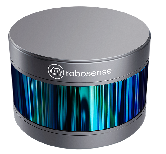
\includegraphics[width=0.15\textwidth]{figures/激光雷达.png}}
	\subfloat[双目深度相机]{%
		\label{fig:rescue_3}
		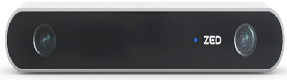
\includegraphics[width=0.25\textwidth]{figures/双目深度相机.png}}
	\subfloat[TOF深度相机]{%
		\label{fig:rescue_2}
		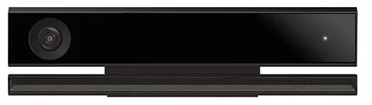
\includegraphics[width=0.25\textwidth]{figures/TOF深度相机.png}}
	\subfloat[结构光深度相机]{%
		\label{fig:rescue_4}
		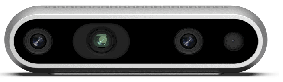
\includegraphics[width=0.25\textwidth]{figures/结构光深度相机.png}}
	\vspace{-1em}
	\caption{常见的三维传感器}
	\label{图:常见的三维传感器}
\end{figure}

激光雷达作为三维传感器中的重要一类,能够通过发射脉冲激光并接收反射信号来构建周围环境的三维点云图像。激光器发射的脉冲光打到物体表面时会发生反射,一部分反射光被激光雷达的接收器捕获,系统通过分析激光脉冲的折返时间,计算出激光雷达到物体的距离。通过多次发射脉冲并逐层扫描目标物体,激光雷达能够生成高精度的三维点云数据,提供目标物体的空间坐标、反射率以及表面纹理等信息。这种高精度的环境建模能力使得激光雷达广泛应用于自动驾驶、无人机导航和机器人环境感知等领域。然而,激光雷达也存在一些限制。首先,其近距离盲区使得在距离较近的环境下,尤其是狭窄的地铁场景中,无法有效探测1米以内的物体。其次,激光雷达生成的点云数据虽然精确,但缺乏颜色和纹理信息,这使得其在特定任务中需要结合其他传感器使用。此外,激光雷达的高成本限制了其在低成本任务中的广泛应用,更适用于开阔的室外场景。

相比之下,RGB-D相机作为一种多模态传感器,结合了RGB相机和深度相机的优势,不仅能够捕获场景中的颜色、纹理等丰富的视觉信息,还能够获取物体的深度数据。RGB相机负责捕捉彩色图像,而深度相机则通过测量每个像素点与相机之间的距离生成深度图像。这种多模态融合的方式为机器人提供了比单一传感器更全面的环境感知能力,使其能够在复杂的地铁环境中进行更加准确的物体识别和空间建模。尽管RGB-D相机的探测距离通常较短,仅在5米范围内有效,但其在近距离环境下表现尤为出色,特别是在地铁车厢等狭小的场景中,RGB-D相机能够捕捉到细节丰富的深度信息。相比于激光雷达,RGB-D相机在处理复杂室内环境时更加灵活且成本更低,成为了室内机器人感知系统的首选。
因此,在地铁排爆任务中,RGB-D相机以其优越的近距离感知能力和对多模态信息的融合,能够帮助救援机器人在复杂环境下实现精确的物体检测、识别和语义分割。通过结合深度学习等先进算法,RGB-D相机能够进一步提高机器人对地铁环境中各种物体的识别精度,帮助其实时、准确地检测出潜在的危险物体,如爆炸物或其他障碍物。这种感知能力的提升不仅显著增强了救援机器人在复杂场景中的任务执行能力,也为机器人自主化作业提供了更坚实的技术支持。


RGB-D相机根据其获取三维数据的方式,主要分为三种类型:被动式、主动式和多模态融合式。这三种方式分别对应不同的技术实现和应用场景。具体来说,目前的商用方案主要包括双目视觉(Stereo Vision)、飞行时间(Time of  Flight, TOF)以及结构光(Structured Light)方案。

在双目视觉方案中,两个类似于人眼间隔排列的RGB相机同时拍摄目标场景,通过基于立体视差原理的特征点匹配技术,计算图像中相应点的位置偏差,进而获得场景的三维几何信息。双目相机的主要优点在于其硬件简单且成本较低,因为其不依赖于外部光源,仅通过图像数据进行处理即可实现三维重建。然而,这种方案也存在显著的局限性。首先,由于该方法完全依赖视觉信息,图像特征点的提取和匹配需要复杂的算法支持,计算量较大,导致实时性较差。其次,RGB相机本身的特性决定了它对纹理单调的场景不适用,当环境中没有足够的图像特征时,匹配精度显著下降,导致深度数据的误差增加​。因此,双目相机在高精度要求的复杂环境中应用有限。目前,国际知名的双目深度相机生产商包括大疆、Intel、Stereolabs和Leap Motion等。

飞行时间(Time of  Flight, TOF)方案则是一种主动式技术。TOF相机通过发射激光脉冲,并通过计算激光脉冲从相机发射到目标表面并返回的时间来确定目标的深度。这种方案的优点在于其探测距离较长,通常可达几十米,尤其适合用于较大的场景或远距离物体的检测。同时,TOF相机在环境光干扰下的表现优异,能够保持较高的成像质量。然而,TOF相机的缺点也比较明显。由于需要连续发射激光脉冲,因此其硬件体积较大,制造成本也较高,这在某些低成本或小型化需求的应用场景中可能成为限制因素。目前,海康威视、联想、Microsoft等公司是TOF相机的主要生产商。

结构光(Structured Light)方案则是通过向目标物体表面投射具有特定结构的红外光图案,并通过接收模组捕捉并解析光图案的反射信息,进而计算物体的三维结构​。结构光相机的精度和分辨率在近距离环境下表现优异,帧率可达60FPS,这使得其非常适用于近距离物体的高精度检测。然而,结构光方案也存在显著的局限性。首先,结构光对环境光线条件十分敏感,在室外或强光环境中,成像效果会大幅下降。其次,随着探测距离的增加,结构光的精度显著下降,因此其不适合远距离物体的检测。目前,奥比中光、Apple、Microsoft和Intel等公司在结构光相机领域具有较大的市场影响力。


三种商用方案的粗略对比如\ref{表:深度相机性能对比} 所示。
\begin{table}[h]
	\caption{深度相机性能对比} % 标题
	\centering % 把表居中
	\renewcommand\arraystretch{1.2}
	\setlength{\tabcolsep}{16pt}
	\footnotesize
	\begin{tabular}{cccc} % 四个c代表该表一共四列,内容全部居中
		\toprule % 第一道横线
		相机类型     & 双目深度相机  & TOF深度相机 & 结构光深度相机 \\
		\midrule % 第二道横线 
		成像原理     & 双目特征匹配  & 飞行时间     & 激光散斑编码 \\
		\specialrule{0em}{1pt}{1pt} 
		分辨率       & 高           & 低          & 中 \\
		\specialrule{0em}{1pt}{1pt}
		成像精度     & 中           & 中          & 中 \\
		\specialrule{0em}{1pt}{1pt}
		制造成本     & 低           & 高          & 中 \\
		\bottomrule % 第三道横线
	\end{tabular}
	\label{表:深度相机性能对比}
\end{table}

通过对双目视觉、结构光以及飞行时间(TOF)三种方案的对比分析可以看出,结构光方案在多个关键方面表现出更为优越的性能。
首先,在环境适应性方面,结构光方案能够较好地应对多种室内环境,尤其是在近距离场景中,结构光技术能够提供高精度的深度感知。相比双目视觉方案,结构光方案通过主动投射特定的光模式,避免了依赖复杂图像特征匹配的过程,因而在纹理不明显或光照条件不佳的环境下依然能够维持较高的深度感知精度。这使得结构光技术在复杂、遮挡严重的环境中表现尤为突出。

此外,结构光在实时性上也表现优异。由于其不需要进行大量的图像特征匹配计算,结构光技术能够快速生成精确的深度图像,使其更适用于需要高实时响应的场景,例如救援机器人在地铁排爆任务中的应用。相比之下,双目视觉方案由于需要较大的计算量来进行图像处理和特征点匹配,实时性较差,难以在动态环境中进行高效的深度感知。
相较于TOF方案,结构光技术还具备较低的功耗优势。TOF技术虽然能够提供远距离的深度感知,但其高功耗和较大的硬件体积限制了其在小型化应用中的使用。同时,结构光技术在当前的发展阶段已相当成熟,具备较高的制造成熟度和相对较低的成本,使其在实际应用中更具竞争力。结构光方案不仅在成本和能耗方面更具优势,还能够满足机器人在狭窄、复杂环境中的操作需求。

基于以上对比分析,本文选择了Intel公司的Realsense D435i作为主要传感器。
Realsense D435i RGB-D相机采用了先进的结构光技术,能够同时获取高质量的彩色图像和深度图像,特别适用于救援机器人在地铁排爆等复杂环境中的实时感知。





\subsection{传统的RGB-D语义分割}
传统的语义分割方法不依赖深度学习,而是采用基于手工设计特征的方案。这类方法通常分为三个阶段:首先是特征选择阶段,研究人员主要依赖于手工设计的特征,例如颜色、纹理和形状等局部外观属性,以及一些常用的局部特征描述子。其次是在分类阶段,这些手工设计的特征被输入到浅层机器学习模型中进行分类,如支持向量机(Support Vector Machine,SVM)和随机森林(Random Forest)等。最后,在结果优化阶段,图模型如马尔可夫随机场(Markov Random Fields,MRF)或条件随机场(Conditional Random Fields,CRF)被用来对分类结果进行进一步优化。虽然传统语义分割方法在某些简单场景下表现良好,但这些方法依赖于人为设计特征,难以适应复杂的环境和多变的视觉特征,因此其适用性在高度复杂的地铁排爆环境中有限。

部分研究致力于改进手工特征的设计,以提高语义分割的精度。例如,Shotton等人\cite{Shotton08CVPR}设计了一种基于低级特征的语义纹理森林(Semantic Texton Forest),实现了语义分割的初步突破。在此基础上,Scharwächter等人\cite{Scharwächter15IVS}联合处理了颜色、纹理和深度信息,利用随机决策森林算法快速推断出街景的粗略布局。这些研究表明,将不同类型的手工设计特征相结合,能够在某种程度上提升语义分割的精度,尤其是在街景和自然场景中。然而,这些方法对手工特征设计依赖较大,难以充分捕捉复杂场景中的高层次语义信息。

尽管基于像素点的传统语义分割方法能够实现一定的目标识别,但其主要问题在于未能有效考虑相邻像素之间的空间关系,容易产生不一致的结果。为了解决这一问题,研究人员提出了基于超像素的方法,该方法通过将局部区域内的像素聚类为超像素,并在相同类别的约束下进行预测,从而提高了分割结果的连续性和一致性。Gupta等人\cite{Gupta15IJCV}通过结合物体外观和几何结构的通用性与特异性特征,设计了一种基于超像素的分类方法,并采用随机森林和SVM模型进一步提升分类的准确性。尽管这些基于手工设计特征的方法在一定程度上改进了分割效果,但其在面对高度复杂的地铁排爆场景时,依然无法与深度学习方法的自适应能力相媲美。

尽管基于超像素的方法在一定程度上增强了像素特征的鲁棒性,通过对局部区域的像素进行聚类,可以有效缓解部分语义分割任务中的不一致问题,但超像素方法在实际应用中依然存在局限。超像素中的像素并不能始终保持完全一致,尤其是在处理复杂或动态环境时,像素特征之间的局部差异仍可能导致分割结果不稳定。为了解决这一问题,研究人员引入了概率图模型以增强分割结果的空间一致性。条件随机场(Conditional Random Field, CRF)作为一种广泛应用的概率图模型,能够通过描述输出标签之间的关系,结合图像特征,优化分割结果。CRF为语义分割提供了一个概率框架,能够有效地将像素之间的空间关系纳入考虑,从而提高分割的连贯性和精确度。

在这一方向上,Ladicky等人\cite{Ladicky10ECCV}针对CRF模型定义了一个全局能量函数,结合了滑动窗口检测器的结果以及基于像素的低级一元和成对关系,成功提升了语义分割的性能。Cadena等人\cite{Cadena14ICRA}则提出了一种有效的策略,通过诱导CRF的图结构来优化推理过程,进一步增强了分割结果的空间一致性。这些改进证明了CRF在语义分割任务中增强空间一致性的重要性,但其对复杂场景的泛化能力依然有限,特别是在面对高度复杂或动态变化的场景时,CRF依赖的人工特征难以全面表达场景的复杂性和多样性。

尽管传统的语义分割方法通过结合超像素和CRF等技术取得了一些进展,但由于这些方法依赖于人工设计的特征,对于处理复杂场景的能力仍存在较大的局限性。手工设计的特征通常无法全面捕捉到场景中的复杂物体和变化环境,特别是在非线性、多尺度的场景下表现尤为不佳。此外,浅层机器学习模型在应对复杂的非线性函数时拟合能力有限,难以有效提取高层次的语义信息。因此,面对复杂的地铁排爆场景等高风险任务,传统语义分割方法的效果很难进一步提升,需要引入更加先进的深度学习技术来实现更高效的语义分割。



\subsection{基于深度学习的RGB-D语义分割}
自Hinton等人\cite{Hinton06Science}在2006年首次提出深度学习(Deep Learning,DL)概念以来,深度学习技术得到了迅速发展,并在计算机视觉领域取得了革命性的突破。在语义分割任务中,传统的基于手工特征的语义分割方法依赖于设计精巧的特征提取算法,但这些方法在处理复杂、多变的场景时,表现出明显的局限性。相比之下,基于深度学习的语义分割方法利用深度神经网络的强大非线性拟合能力,能够自动从大量数据中学习到高级语义特征,极大地提高了图像理解的准确性和鲁棒性。

深度神经网络通过层层卷积的结构,逐步从低层次的像素信息提取出高层次的语义信息,这使得网络不仅能够识别图像中的基本元素,还能在复杂场景中准确地解析不同物体的边界和类别。与传统的语义分割方法相比,深度学习方法具备显著优势:它能够自动学习图像中的重要特征,无需依赖手工设计的特征提取步骤。此外,深度学习还能够处理更大规模的数据集,使得训练模型能够更好地泛化到复杂、真实的应用场景中,如地铁排爆环境中的救援机器人任务。


\subsubsection{基于卷积神经网络的RGB-D语义分割}
卷积神经网络(Convolutional Neural Network, CNN)的出现,极大地提升了语义分割的性能,并为复杂场景下的图像处理提供了强有力的工具。Long等人\cite{Long15CVPR}提出的全卷积神经网络(Fully Convolutional Network, FCN),首次将深度学习技术引入语义分割领域,开创了图像语义分割的新时代。FCN通过将传统卷积神经网络中的全连接层替换为卷积层,转变为可以用于像素级分类的分割网络,能够对图像中的每个像素进行语义标注。这一创新设计显著提高了网络的分割性能,并通过使用转置卷积层(deconvolution layers)进行上采样,使得网络能够在保持原有分辨率的同时,生成高精度的分割结果。FCN还具备处理任意大小图像的能力,极大地提升了语义分割的计算效率。由于这一技术首次实现了从端到端对图像进行训练,后续的大多数语义分割研究几乎都基于FCN的基础架构进行改进和优化。

针对RGB-D双模态的语义分割,研究人员也探索了多种深度学习的融合方案。Couprie等人\cite{Couprie14MLR}提出了一种前融合(Early Fusion)方案,其基本思想是将RGB图像和深度图像逐帧分解后,拼接为四通道的输入数据,并输入到卷积神经网络中进行处理。这种方法实现了对视频流的RGB-D实时语义分割,但其主要问题在于RGB和深度数据的模态差异没有得到充分利用,导致网络难以区分两者的特性信息,因此可能在某些场景下降低了分割精度。然而,上述策略(如前融合策略)主要是直接融合采集到的图片数据信息,虽然实现了基本的融合操作,但这类策略往往缺乏对不同模态数据的特征提取过程,通常无法兼顾最优分割性能。为了弥补这一不足,Hazirbas等人在2016年提出了一种基于双流网络进行间接特征融合的RGB-D语义分割网络FuseNet。FuseNet通过设计一种编解码结构,将深度通道和图像通道之间添加中间特征映射,提升了多模态数据的互补效果,进而获得了更为理想的融合性能。同年,Li等人提出了一种长短期记忆(Long Short-Term Memorized Context Fusion,LSTM-CF)网络模型,该方法通过水平和垂直的多向融合实现全局上下文信息的整合,显著提高了RGB-D语义分割的准确性 。

为了更好地利用深度信息,Gupta等人\cite{Gupta14ECCV}提出了一种基于编码的深度数据处理方案,将深度图像编码为三个通道,分别包含水平视差(Horizontal disparity)、地面高度(Height above ground)和重力夹角(The angle between the pixel’s local surface normal and the inferred gravity direction)等信息。这一编码方案有效地增强了网络对深度信息的利用,能够显著提升语义分割的精度和鲁棒性,特别是在处理复杂三维场景时。然而,这种方法的不足之处在于它需要获取额外的相机位姿数据,并且编码过程计算代价较高,在实时性要求较高的任务中可能存在一定的局限性。

针对深度几何信息在固定卷积神经网络上表现有限的问题,Wang等人在2018年提出了深度感知卷积和深度感知平均池化算子,以提高对两种模态数据的处理效果。Jiang等人提出的对称残差编解码网络则通过深度编码器和解码器结构,解决了小目标融合难的问题 。近年来,RGB-D语义分割技术不断在网络结构优化方面取得进展。例如,Jiao等人提出了一个引入深度几何信息的语义分割框架,并通过跳跃金字塔模块提升上下文融合效果 。Hu等人则引入注意力机制,提出了三分支网络模型ACNet,显著改善了RGB-D数据的深度融合效果 。2021年,Chen等人提出的GLPNet模型通过局部和全局上下文融合模块,进一步推动了RGB-D语义分割的前沿发展。随着深度学习技术的快速发展,RGB-D语义分割的融合方式逐渐从早期的简单拼接模式,向更复杂的模态融合策略演进。一些研究开始引入注意力机制,通过权重分配来增强不同模态之间的互补信息利用,这进一步提高了救援机器人在复杂环境中的场景理解能力。

















\iffalse 
上述策略都是围绕直接融合采集到的图片数据信息而提出的,即前融合策略, 但这类策略缺乏对不同模态数据的特征提取过程,通常无法兼具最优分割性能。

为了避免这一问题,Hazirbas等人在201 6年提出了一种基于双流网络进行间接特征融合的RGBD语义分割网络FuseNet[ 22],该方法设计了一种图像语义分割的编解码结构,通过在深度通道和图像通道之间添加中间特征映射,提升多模态数据的互补,获得了更好的融合效果。
同年,Li等人提出了一种新型(Long Short-Term Memorized Context Fusion,LSTM-CF)的网络模型[ 23],如图1.9所示,该方法通过水平和垂直多向融合实现全局上下文信息的整合,较好的利用了图像和深度的相关性,提高了语义分割的正确率。 


Long等人将其扩展到了RGB-D数据上:训练两个FCN网络,用来分别处理彩色图像和深度图像;再将两个网络的预测求和,得到最终的分类结果。为了提高融合的效率,Cheng等人设计了门控融合层来自动的学习高层的模态特异的特征[ 68]。
层次融合方法[ 66,71–74]可以在多个不同的层融合两个模态的特征。


FuseNet [71]以自底向上方式将多层的深度特征融入到RGB编码器。
RedNet[ 72]扩展了FuseNet,在自顶向下的路径上融合两个模态的多层特征。
SSMA[ 66]提出了一个自监督的模型适应融合机制(SSMA)来融合模态特征的特征,也是在自顶向下的路径上融合多层的特征。


例如,2017年Lee等人提出的RDFN et网络模型[ 24],就是基于当年里程碑式的RefineNet网络[ 25]而推广提出的。该网络较好的继承了残差学习机制, 通过MMFNet模块和多个RefineNet模块跳跃连接方式,细化图像和深度的融合方式,在试验验证中取得了较好的表现。

同年,Qi等人提出一种基于3D图网络的语义分割新网络模型3DGNN[26],通过将二维图像和深度信息融合,得到对应点的空间三维坐标(x,y,z),有效的减少了图片距离误导的错误发生,但在复杂场景或者二维/三维上下文相似场景中,也容易产生一定的误判。

同年,Schneider等人提出[ 27]了一种基于独立分支的RGBD中层特征融合模型,该方法具有较强的扩展性, 可通过简单的调整适用不同模态数据的处理,在公开数据集上保持了较高的性能指标。

针对深度几何信息在固定卷积神经网络上效果有限的问题,201 8年,Wang等人提出了深度感知卷积和深度感知平均池化[ 28]的算子,在不增加网络计算量的前提下,提高模型对两种模态数据的兼顾性,但实验结果表明这类方法对小目标的效果有限,需要在多尺度处理上进行改进。

同年,Jiang等人提出了一个对称的残差编解码网络[ 29],该网络深度很深却解决了细节遗失和梯度消失的问题,在小目标融合的效果上有显著提升。

近三年,基于深度学习的RGBD算法改进主要是针对语义特征提取网络的优化工作。
2019年Jiao等人提出了深度几何信息引入辅助语义分割的网络框架[ 30],该网络将骨干网络的权值相互分享,改进语义特征,并使用跳跃金字塔模块,提升上下文融合效果。

同年,Hu等人融入了注意力机制,提出了三平行分支架构的网络模型ACNet[ 3 1],充分融合深浅层特征,平衡图片和深度的作用比重,如图1.10 所示。

为了进一步充分利用两者互补性,在2020年北大、商汤科技、港大联合提出了一种引入作用于特征分离和聚合的注意力机制的网络模型[ 32],是互补信息重新校准融合。

2021年Chen等人提出的GLPNet网络[ 33]成功地在较深阶段保持两种信息稳定地传播,其原因在于引入局部上下文融合模块(L-CFM)进行动态对齐,引入全局上下文融合模块(G-CFM)进行联合建模。
\fi



 %\cite{Gupta14lECCV}





\subsubsection{基于transformer的RGB-D语义分割}
近年来,Transformer模型在自然语言处理领域取得了巨大的成功,并且其自注意力机制(Self-Attention Mechanism)在图像处理中展现出强大的特征提取能力。与传统的卷积神经网络(CNN)不同,Transformer通过全局建模图像中的像素关系,能够更好地捕捉长距离依赖和全局上下文信息。这使得其在高复杂度、多模态的语义分割任务中展现出极大的潜力。
基于Transformer的RGB-D语义分割模型开始逐步取代基于卷积的模型,成为该领域新的研究热点。与传统的基于CNN的模型相比,Transformer不仅能够通过自注意力机制实现全局范围内的信息交互,还能够通过并行化计算加速特征的提取和融合。尤其是在RGB-D语义分割任务中,Transformer能够更好地处理RGB图像中的纹理信息和深度图像中的几何信息的融合问题,弥补了CNN在多模态特征融合上的局限性。

目前,许多研究者开始探索如何将Transformer架构应用于RGB-D语义分割任务中。例如,Dosovitskiy等人提出的ViT(Vision Transformer)模型,首次将Transformer用于图像处理,是第一个将纯Transformer结构引入视觉任务的模型。ViT通过将图像分割为固定大小的16×16像素的图像块(patches),并将这些图像块作为输入,利用Transformer的自注意力机制来捕捉全局特征 。然而,ViT最初仅应用于标准的RGB图像分类任务,在RGB-D语义分割中未能充分考虑深度信息。尽管如此,ViT的提出为Transformer在图像处理中的应用奠定了基础,并激发了后续基于Transformer的RGB-D语义分割研究。
% Dosovitskiy, A., et al. (2020). "An Image is Worth 16x16 Words: Transformers for Image Recognition at Scale." 

Zheng等人随后提出了SETR(Segmentation Transformer),该模型通过将Transformer应用于图像语义分割任务,彻底摆脱了传统CNN的结构。SETR将Transformer作为特征提取器,并通过上采样层对分割图进行重建。这一模型表明,Transformer不仅在分类任务中有效,在复杂的像素级任务(如语义分割)中也具有巨大潜力 。然而,SETR仍然主要针对RGB图像,未能深入处理RGB-D数据。针对这一挑战,Liu等人提出了RGB-D Transformer语义分割模型,这是专门为处理RGB和深度图像的语义分割任务设计的。该模型通过独立处理RGB和深度通道,并通过中间层的特征融合机制,充分利用Transformer捕捉长距离依赖的能力。
与此同时,Chu等人提出了Twins Transformer,该模型通过局部和全局注意力机制的结合,解决了标准ViT在大规模图像处理时的计算效率问题。Twins Transformer引入了两个分支,一个处理局部信息,另一个处理全局上下文信息,这使得该模型能够在语义分割任务中同时捕捉到细节和全局特征 。尽管Twins Transformer的研究重点在RGB图像上,但其结构和注意力机制为RGB-D语义分割任务提供了重要的借鉴。
除了传统的Transformer架构外,一些研究者还提出了创新的网络设计。Jiang等人在2018年提出了RedNet,这是一种基于深度学习的RGB-D语义分割网络,结合了残差网络(ResNet)和双流网络的优势。RedNet使用两个独立的编码器来处理RGB和深度数据,并在解码阶段进行特征融合。该方法通过残差连接来减轻梯度消失问题,同时有效融合了RGB和深度特征,使得模型能够在复杂环境下(如地铁排爆场景)进行高精度的分割。
Hu等人提出的ACNet(Attention Complementary Network)模型通过引入三分支结构来处理RGB和深度图像的特征。ACNet采用了注意力机制,以自适应地调整RGB和深度特征之间的权重分配,从而更好地融合这两类信息。该模型在多个RGB-D语义分割任务中表现出色,尤其是在复杂的室内和室外场景中。ACNet的研究表明,注意力机制能够有效增强RGB-D语义分割的性能,并在地铁排爆等复杂任务中发挥重要作用。

此外,为了进一步提升Transformer在RGB-D语义分割中的性能,近年来的研究中还引入了多模态融合机制。Zhang提出的Trans4Trans模型专注于透明物体分割,通过多模态特征融合,展示了Transformer在处理复杂RGB-D任务中的潜力。Transformer的RGB-D语义分割研究取得了显著的进展,但在应用过程中仍面临一些挑战。首先,Transformer的高计算成本和内存需求限制了其在实际场景中的广泛应用,特别是在资源有限的移动机器人系统中。其次,如何在更深层次上融合RGB和深度数据,提升多模态信息的互补性,依然是未来研究的一个重要方向。
综上所述,基于Transformer的RGB-D语义分割技术凭借其在长距离依赖建模和全局特征提取方面的优势,展现出了极大的应用潜力。随着深度学习和自注意力机制的进展,RGB-D语义分割技术正朝着更高精度、更强鲁棒性和更广泛应用的方向发展,Transformer架构的不断优化及其在多模态融合策略上的改进,未来该技术将在救援机器人、自动驾驶、安防监控等领域发挥更加重要的作用。


(我就不插参考文献了,给你列在这里,方便你调整和插:

Zheng, S., et al. (2021). "Rethinking Semantic Segmentation from a Sequence-to-Sequence Perspective with Transformers." Proceedings of the IEEE/CVF Conference on Computer Vision and Pattern Recognition (CVPR).

Liu., et al. (2021). "SwinNet: Swin transformer drives edge-aware RGB-D and RGB-T salient object detection" 

Chu, X., et al. (2021). "Twins: Revisiting the Design of Spatial Attention in Vision Transformers." 

Jiang, J., et al. (2018). "RedNet: Residual Encoder-Decoder Network for Indoor RGB-D Semantic Segmentation."

Hu, X., et al. (2019). "Acnet: Attention based network to exploit complementary features for rgbd semantic segmentation." 

Zhang, J., et al. (2021). "Trans4Trans: Efficient transformer for transparent object segmentation to help visually impaired people navigate in the real world")


\subsubsection{基于mamba的RGB-D语义分割}
基于Mamba的RGB-D语义分割是一种新兴的技术,它结合了RGB图像的丰富色彩信息和深度图的精确空间信息,以提高对复杂场景的理解能力。Mamba架构以其高效的全局上下文建模能力在遥感图像处理中显示出巨大的潜力,尤其是在处理大规模场景时。Mamba架构的核心是选择性结构化状态空间模型(SSM),它能够在保持线性时间复杂度的同时捕获长距离依赖性。与传统的卷积神经网络(CNN)相比,Mamba能够更有效地处理全局上下文信息,而与基于Transformer的方法相比,Mamba避免了高计算复杂性。在RGB-D语义分割领域,Mamba的应用还处于起步阶段,但已有一些创新的研究工作。例如,Sigma模型采用了Mamba架构进行多模态融合,通过编码器和创新的Mamba融合机制,有效地从不同模态中提取关键信息,并在RGB-热成像和RGB-深度分割任务上展示了优越的性能。

Zhong等人[XXX]提出了一种基于注意力机制的融合网络,用于RGB-D语义分割。该网络采用了前向多步传播策略和后向渐进自举融合策略,通过在不同尺度上聚合特征图,有效减少了最终预测中的不确定性。此外,引入了通道和空间校正模块(CSRM),以实现多维交互和噪声去除。通过交叉注意力融合模块(CAFM),实现了RGB和深度图像之间的全面融合。在室内NYU Depth V2和SUN-RGBD数据集上进行了广泛的实验,证明了该网络能够巧妙地处理多种复杂场景。
Ding等人[]提出了一种名为RTMamba的新架构,用于实时遥感语义分割任务。该架构包括一个主干网络、一个解码器和一个语义变换器。主干网络利用CNN进行浅层特征捕获,并使用视觉状态空间模型(VSS)块来捕获深层特征和长距离依赖性,从而降低计算复杂性。解码器预测特征掩模,并包括一个倒置三角形金字塔池化(ITP)模块,用于过滤冗余信息并增强多尺度目标感知。在训练期间,语义变换器仅用于提供语义和空间细节信息,以辅助主干网络和解码器。在推理期间,RTMamba仅保留主干网络和解码器,确保了轻量级架构。
Wan等人[]引入了Sigma,这是一个用于多模态语义分割的Mamba网络,利用选择性结构化状态空间模型(Mamba)。Sigma通过暹罗编码器和创新的Mamba融合机制,有效地从不同模态中选择重要信息。然后开发了一个解码器,以增强模型的通道建模能力。Sigma在RGB-热成像和RGB-深度分割任务上进行了严格的评估,展示了其优越性,并标志着状态空间模型(SSMs)在多模态感知任务中的首次成功应用。

这些研究展示了基于Mamba的RGB-D语义分割方法的在网络架构的创新、注意力机制的应用、以及多模态数据融合策略的发展现状。基于Mamba的RGB-D语义分割方法的研究不仅推动了RGB-D语义分割技术的发展,也为机器人导航、自动驾驶、室内建模等领域的应用提供了新的可能性,但也仍然在多模态融合、计算效率和泛化能力上面临一些挑战,如何设计更有效的融合策略以充分利用RGB和深度信息的互补性,在保持高性能的同时如何降低计算复杂度以便在资源受限的机器人上部署,以及如何提高模型在不同地铁场景和数据集之间的泛化能力,是值得关注和研究的重点。

(我就不插参考文献了,给你列在这里,方便你调整和插:
Zhong   Attention-based fusion network for RGB-D semantic segmentation
Ding    A Novel Mamba Architecture with a Semantic Transformer for Efficient Real-Time Remote Sensing Semantic Segmentation
Wan    Sigma: Siamese Mamba Network for Multi-Modal Semantic Segmentation
)



\section{主要研究内容与论文组织结构}


\subsection{主要研究内容}

\subsection{论文组织结构}




